% ====================================================================
%+
% SECTION:
%    grb.tex
%
% CHAPTER:
%    transients.tex
%
% ELEVATOR PITCH:
%-
% ====================================================================

\section{Gamma-Ray Burst Afterglows}
\def\secname{\chpname:grbs}\label{sec:\secname}

\credit{ebellm}

Gamma-ray bursts (GRBs) are relativistic explosions typically classified
by the temporal duration of their initial gamma-ray emission: Long GRBs,
that mark the endpoint of the lives of some massive stars, and short
GRBs, believed to originate from the merger of binary neutron stars. GRB
emission is known to be beamed: the initial prompt gamma-ray emission is
seen only for observers looking at the jet axis. The longer-wavelength
X-ray, optical, and radio afterglow may be seen both by on- and off-axis
observers.  The latter case is known as an orphan afterglow, due to the
absence of gamma-ray emission. On- and off-axis afterglows are predicted
to have different temporal signatures in the optical: On-axis events
decay as a power-law until a jet break, while off-axis events should be
fainter and show an initial rise (Figure \ref{fig:afterglow_lcs}).
Despite systematic searches, no convincing orphan afterglow candidates
have yet been discovered, limiting our knowledge of the beaming fraction
of GRBs and hence their true rates. Well-sampled orphan afterglow
lightcurves would also permit study of the GRB jet structure.

\begin{figure}[hbt]
\centerline{
\includegraphics[width=0.6\textwidth]{figs/transients/predicted_afterglow_lcs_mag.pdf}
}
\caption{ Predicted light curves of GRB afterglows by off-axis angle
with respect to the jet axis $\theta_{\rm obs}$ \citep[Figure
8.8,][]{2009arXiv0912.0201L}. The forward shock model is derived from
\citet{2002ApJ...576..120T} and assumes a jet half opening angle
$\theta_j = 4^\circ$, the isotropic equivalent energy of $E_{\rm iso} =
5\times10^{53} \rm erg$, ambient medium density $n = 1$ g cm$^{-3}$, and
the slope of the electron energy distribution $\rm p = 2.1$. The
apparent AB $r$-band magnitudes assume a source redshift $z = 1$. }
\label{fig:afterglow_lcs}
\end{figure}

Because of their rarity, in all but one case \citep{2015ApJ...803L..24C}
to date GRBs have been discovered using their prompt emission by hard
X-ray or gamma-ray all-sky monitors. This selection imposes biases on
the population of relativistic explosions we observe. Baryon-loading in
the GRB jet---a ``dirty fireball'' \citep{2003ApJ...591.1097R}---can
lead to on-axis events without gamma-ray emission.  Only one plausible
candidate has been identified to date \citep{2013ApJ...769..130C}.
Discovery of new dirty fireballs---if distinguished from off-axis
events--would clarify the rates of these events and enhance our
understanding of the diversity of stellar death.

LSST is the survey most capable of resolving these decades-old
questions.  Due to its large aperture and etendue, LSST can detect
faint, fast-fading, and rare cosmological events, potentially enabling
population studies of the high-redshift universe.
\citet{2015A&A...578A..71G} estimated LSST could detect 50 orphan
afterglows each year, more than any other planned survey.

%deep survey helps due to time dilation

%beaming fraction and true rates; jet structure; dirty fireballs?
%GRB-SN connection; probe high-z star formation?

%other fast transients: Fast transients and SN shock breakout?  flash spectroscopy

The challenge of detecting and recognizing GRB afterglows in the LSST data in
real time makes this science case a useful proxy for other fast transient
science cases that benefit from $N > 2$ visits per night.  In particular, this
includes discovering supernovae soon after explosion for flash spectroscopy or
shock breakout searches.

% need appropriate cadences to support value of realtime alert stream

% --------------------------------------------------------------------

\subsection{Target measurements and discoveries}
\label{sec:\secname:targets}

GRB afterglow discovery is among the science cases that places the
greatest stress on the LSST cadence.  Because afterglows fade
rapidly---dropping several magnitudes in the first few hours---high
cadence observations are required to detect the fast fading. If an
afterglow candidate can be recognized in real time, it will be possible
to trigger TOO spectroscopy (to measure a redshift and confirm the event
is cosmological), X-ray and radio observations (to detect a high-energy
counterpart and the presence of a jet), and additional photometry (to
characterize the lightcurve evolution).  If there is no source at the
location of the transient in the coadded reference image, two
consecutive observations in the same filter separated by an hour or two
are the minimum required to potentially trigger followup of a
fast-fading event. However, a third observation within a night or
two---ideally in the same filter---would improve the purity of the
sample and reduce the reliance on triggered followup. Observations in
other bands at high cadence are less useful because they require
assumptions about the event's SED and its evolution to determine if a
source is truly fading.

Distinguishing orphan afterglows from on-axis events (whether conventional
GRBs or dirty fireballs) will also require more than two detections.
Orphan events may prove harder to recognize in real time, because they are
intrinsically fainter than on-axis events and show an initial rise rather
than a rapid decay (Figure \ref{fig:afterglow_lcs}).  Additionally, because
of relativistic time dilation, high redshift events are easier to detect,
but these events will be fainter and more difficult to follow up.
Accordingly, population studies of orphan afterglow candidates may by
necessity be conducted with LSST photometry alone.  Such studies may only
be productive if LSST has sufficiently frequent revisits to a field in a
single filter.

% --------------------------------------------------------------------

\subsection{Metrics}
\label{sec:\secname:metrics}

The core figure of merit for GRB afterglows is simply the raw number of
on- and off-axis events detectable in two, three, or more observations,
preferably in a single filter.

The appropriate way to derive these detections is to conduct a Monte
Carlo simulation of a cosmological population of GRBs and fold it
through the LSST observing cadence \citep[cf.][]{2011PASP..123.1034J}.
We are developing this infrastructure for the MAF framework.

In the meantime, simplified metrics can give us a general idea of how well
a given cadence can characterize fast-evolving transients such as GRBs.  We
have created a new metric, \texttt{GRBTransientMetric}, that replaces the
linearly rising and decaying lightcurve in \texttt{TransientMetric} with
the $F \sim t^{-\alpha}$ decay characteristic of on-axis afterglows.  (For
the time being, we neglect the jet break that steepens the rate of decay;
this implies that our detectability estimates are optimistic.)

We simulate random on-axis afterglows using the parameters of
\citet{2011PASP..123.1034J}: the R-band apparent magnitude at 1 minute
after explosion is randomly drawn from a Gaussian with $\mu=15.35$,
$\sigma=1.59$ and decays with $\alpha=1.0$.  For these estimates we
simply assume zero color difference between in all LSST bands.
There are roughly 300 on-axis GRBs per year with these parameters;
we calculate the average fraction of these events which have at least one,
two, or three detections in any single filter.

% Can use https://github.com/lsst/sims_maf/blob/master/python/lsst/sims/maf/metrics/tgaps.py or https://github.com/lsst/sims_maf/blob/master/python/lsst/sims/maf/metrics/cadenceMetrics.py (Inter/Intra-night) to get histograms.  Would be nice to extend to single-band, N-offset

% --------------------------------------------------------------------

\subsection{OpSim Analysis}
\label{sec:\secname:analysis}

We ran \texttt{GRBTransientMetric} on several OpSim v3.3.5 runs with a range of
characteristics:  \opsimdbref{db:baseCadence}, the baseline cadence;
\opsimdbref{db:NEOswithVisitTriplets}, with three visits per WFD field;
\opsimdbref{db:NoVisitPairs}, with no visit pairs; and
\opsimdbref{db:opstwoPS}, a PanSTARRS-like cadence.

\autoref{tab:SummaryGRBs} lists the fraction of on-axis afterglows
detected in at least one, two, and three visits in a single filter.

Because of its wider areal coverage, the PanSTARRS-like cadence of
\opsimdbref{db:opstwoPS} maximizes the fraction of events detected in
one and two epochs.  Not surprisingly, the triplet-visit WFD cadence of
\opsimdbref{db:NEOswithVisitTriplets} maximizes the three-epoch detection
rate.


\begin{table}
  \begin{tabular}{l|p{6cm}|c|c|c|c|p{5cm}}
    FoM & Brief description & {\rotatebox{90}{\opsimdbref{db:baseCadence}}}
	  & {\rotatebox{90}{\opsimdbref{db:NEOswithVisitTriplets}}} &
	  {\rotatebox{90}{\opsimdbref{db:NoVisitPairs}}} &
	  {\rotatebox{90}{\opsimdbref{db:opstwoPS}}} & Notes \\
    \hline
    \thesection-1 & \footnotesize{\texttt{GRBTransientMetric},
    \texttt{nPerFilter}\,$=1$}      & 0.17 & 0.16 & 0.20 & \textbf{0.21} &
    \footnotesize{Fraction of GRB-like transients detected in at least one
    epoch.} \\
    \thesection-2     & \footnotesize{\texttt{GRBTransientMetric},
    \texttt{nPerFilter}\,$=2$}      & 0.12 & 0.10 & 0.09 & \textbf{0.14} &
    \footnotesize{Fraction of GRB-like transients detected in at least two
    epochs in any single filter.} \\
    \thesection-3     & \footnotesize{\texttt{GRBTransientMetric},
    \texttt{nPerFilter}\,$=3$}      & 0.05 & \textbf{0.08} & 0.04 & 0.04 &
    \footnotesize{Fraction of GRB-like transients detected in at least
	    three epochs in any single filter.}
\end{tabular}
\caption{Mean figures-of-merit (FoMs) for on-axis Gamma-Ray Bursts for one,
two, and three detections in a filter.
The best value of each FoM is indicated in bold.
The wider areal coverage of \opsimdbref{db:opstwoPS} improves its detection
rate of GRBs in one and two epochs, while the triplet visits
in \opsimdbref{db:NEOswithVisitTriplets} naturally improve the
three-detection efficiency.
}
\label{tab:SummaryGRBs}
\end{table}

% --------------------------------------------------------------------

\subsection{Discussion}
\label{sec:\secname:discussion}

An LSST cadence purely designed for discovering GRB afterglows would
include three or more visits to each field every night, with the visits
separated by an hour or two. Moreover, it would be conducted in a single
filter in order to best identify the lightcurve shape of off-axis
events.

While the current surveys simulated are far from this ideal
(usually just two closely spaced visits, with subsequent revisits days
later), nonetheless an appreciable number of GRBs are detectable.
\opsimdbref{db:NEOswithVisitTriplets} would detect about 25 events each
year in three epochs, already potentially the largest sample of untriggered
afterglows.

However, some care is required in interpreting these values:
while the GRB afterglow fades rapidly over the first day of the explosion
(Figure \ref{fig:afterglow_lcs}), at later times a 30 minute visit
separation is not enough to reveal significant evolution in the lightcurve.
We intend to enhance our metric to require that detections are counted only
if significant evolution is statistically distinguishable with 1\%
photometry.

In future work we intend to simulate cosmological populations of on- and
off-axis in order to better determine how many events could be discovered
in time to trigger real-time followup\footnote{or conversely, 
constrain the area
over which high-cadence observations are required to detect a meaningful
population of GRBs.}.

\begin{figure}[hbt]
\centerline{
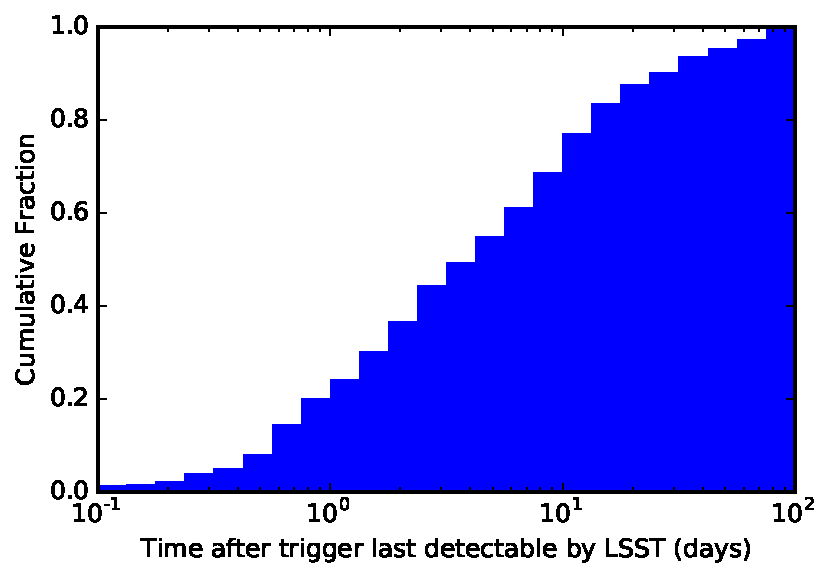
\includegraphics[width=0.6\textwidth]{figs/transients/afterglow_cdf.pdf}
}
\caption{ Cumulative fraction of GRB on-axis afterglows fainter than
magnitude 24.7 at a given time after the burst. We use an $\alpha=1$
decay with no jet breaks and the brightness parameters of
\citet{2011PASP..123.1034J}. }
\label{fig:afterglow_visibility}
\end{figure}

Thanks to LSST's depth, GRBs can be visible for weeks (Figure
\ref{fig:afterglow_visibility}).  Accordingly,
modest enhancements to the intra- and inter-night revisit rate with
single-filter rolling cadences should substantially improve LSST's
discovery and characterization of relativistic explosions.


\subsection{Conclusions}

Here we answer the ten questions posed in
\autoref{sec:intro:evaluation:caseConclusions}:

\begin{description}

\item[Q1:] {\it Does the science case place any constraints on the
tradeoff between the sky coverage and coadded depth? For example, should
the sky coverage be maximized (to $\sim$30,000 deg$^2$, as e.g., in
Pan-STARRS) or the number of detected galaxies (the current baseline 
of 18,000 deg$^2$)?}

\item[A1:] No strong constraint, although on average
	larger sky coverage provides fewer epochs for the dense time sampling
	required to detect fast-fading events like GRBs.

\item[Q2:] {\it Does the science case place any constraints on the
tradeoff between uniformity of sampling and frequency of  sampling? For
example, a rolling cadence can provide enhanced sample rates over a part
of the survey or the entire survey for a designated time at the cost of
reduced sample rate the rest of the time (while maintaining the nominal
total visit counts).}

\item[A2:]  Frequency of sampling is far more important than uniformity of
	sampling for fast transients like GRBs.  Rolling cadences with
		three or more epochs per night or two are needed for
		realtime discovery of young events.

\item[Q3:] {\it Does the science case place any constraints on the
tradeoff between the single-visit depth and the number of visits
(especially in the $u$-band where longer exposures would minimize the
impact of the readout noise)?}

\item[A3:]  While greater single visit depth probes a greater cosmological
	volume within which to detect GRBs and other fast transients,
		our efficiency at discovering
		GRBs with LSST is driven entirely by the time sampling.
		Accordingly we prefer a larger number of visits per field
		to greater single-exposure depth, independent of band..

\item[Q4:] {\it Does the science case place any constraints on the
Galactic plane coverage (spatial coverage, temporal sampling, visits per
band)?}

\item[A4:] As GRBs are cosmological events, we expect to detect very few at
	low Galactic latitudes due to extinction.  Accordingly this
		science case is insensitive to observing plans in the Plane
		except insofar as they limit the number and cadence of
		exposures at higher latitudes.

\item[Q5:] {\it Does the science case place any constraints on the
fraction of observing time allocated to each band?}

\item[A5:] No strong constraints, although detection of faint afterglows
	will benefit from exposures taken in the bands with deepest
		single-exposure depth.

\item[Q6:] {\it Does the science case place any constraints on the
cadence for deep drilling fields?}

\item[A6:] Deep drilling fields provide an excellent opportunity to achieve
	the high time sampling required to discover GRBs while they are
		young.  As discussed above, a good fast transient cadence
		might have a \textit{minimum} of three visits
		in a night separated by an hour or two, preferably in a
		single filter, with revisits every night.

\item[Q7:] {\it Assuming two visits per night, would the science case
benefit if they are obtained in the same band or not?}

\item[A7:] Due to the need to constrain the lightcurve shape, it is best if
	the observations are in the same filter--especially with only two
	visits per night.  Otherwise there is a degeneracy between the
	(evolving) color of the event and its lightcurve shape.

\item[Q8:] {\it Will the case science benefit from a special cadence
prescription during commissioning or early in the survey, such as:
acquiring a full 10-year count of visits for a small area (either in all
the bands or in a  selected set); a greatly enhanced cadence for a small
area?}

\item[A8:] A dedicated experiment providing enhanced cadences over a small
	area  (as described above) would provide an ideal
	experiment to determine the rate of fast transients.  Such an
	observing strategy would also
	facilitate organizing necessary followup resources
	(spectroscopy, X-ray followup) because the observing period would
	be known in advance.

\item[Q9:] {\it Does the science case place any constraints on the
sampling of observing conditions (e.g., seeing, dark sky, airmass),
possibly as a function of band, etc.?}

\item[A9:] None unique to the science.

\item[Q10:] {\it Does the case have science drivers that would require
real-time exposure time optimization to obtain nearly constant
single-visit limiting depth?}

\item[A10:] No.

\end{description}

\navigationbar
